\documentclass[journal,12pt,twocolumn]{IEEEtran}
\usepackage[utf8]{inputenc}
\usepackage{amsmath}
\usepackage{amssymb}
\usepackage{graphicx}
\providecommand{\brak}[1]{\ensuremath{\left(#1\right)}}

\title{Assignment 2}
\author{ADEPU VASISHT}
\date{March 2021}

\begin{document}

\maketitle

\section*{GATE EC Problem 30}
If E denotes the expectation, the variance of a random variable X is given by ?

\begin{description}
\item[$\brak{A}$]$E[X^2]-E^2[X]$ 
\item[$\brak{B}$]$E[X^2]$
\item[$\brak{C}$]$E[X^2]+E^2[X]$ 
\item[$\brak{D}$]$E^2[X]$
\end{description}
\section*{Solution}
The expectation of a random variable X is given by $$E[X]=\sum_{all \ x}x\Pr\brak{x}$$
The expectation of a random variable is also known as mean of random variable and denoted as $\mu$\\\\
The expectation of a function $g\brak{X}$ is given by $$E[g\brak{X}]\sum_{all \ x}g\brak{x}\Pr\brak{x}$$

The variance of a random variable $X$ is given as $$Var\brak{X}=E[\brak{X-\mu}^2]$$

We know that



\begin{align}
    E[\brak{X-\mu}] &= \sum_{all \ x} \brak{x-\mu}^2 \Pr\brak{x}\\
    E[\brak{X-\mu}] &= \sum_{all \ x} \brak{x^2-2\mu x+\mu^2} \Pr\brak{x}\\
    &= \sum_{all \ x}x^2\Pr\brak{x}-2\mu\sum_{all\ x}x\Pr\brak{x}+\mu^2\sum_{all\ x}\Pr\brak{x}\\
    &= E[X^2]-2\mu.\mu+\mu^2\brak{1}\\
    &= E[X^2]-\mu^2\\
    &= E[X^2]-E^2[X]
\end{align}

$$\therefore$$ Hence option A is the correct answer

\section*{The python codes}
We run a simulation using binomial distribution with random probabilities and random number of values the random variable can take. We then plot variance calculated using the above formula on the X-axis while on the Y-axis we use variance from the inbuilt function inside the scipy library. If the formula is correct then the plotted points should be around the x=y line. The graph is shown below.

\begin{figure}[h]
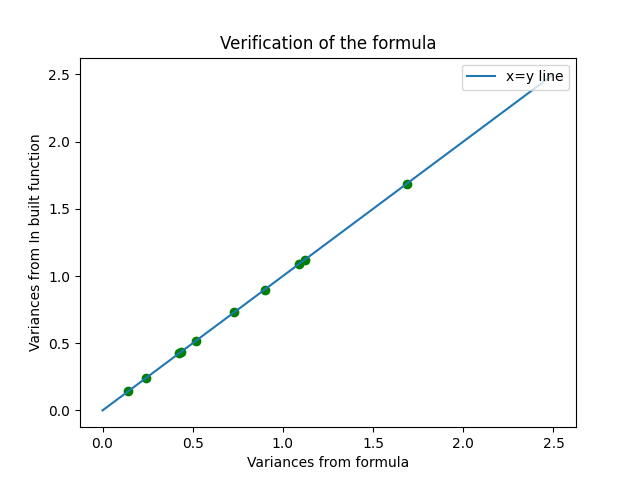
\includegraphics[scale = 0.7]{ogimage}]
\end{figure}





\end{document}